\documentclass[11pt,a4paper]{article}

\usepackage[utf8]{inputenc}
\usepackage[T1]{fontenc}
\usepackage[english]{babel}
\usepackage{geometry}
\geometry{top=2.5cm, bottom=2.5cm, left=2.5cm, right=2.5cm}
\usepackage{fancyhdr}
\usepackage{lastpage}
\usepackage{booktabs}
\usepackage{tabularx}
\usepackage{longtable}
\usepackage{float}
\usepackage{graphicx}
\usepackage{xcolor}
\usepackage{hyperref}
\usepackage{listings}
\usepackage{enumitem}
\usepackage{amsmath,amssymb}
\usepackage{microtype}
\usepackage{tikz}
\usepackage{pgfplots}
\pgfplotsset{compat=1.18}
\usetikzlibrary{shapes.geometric, arrows.meta, positioning, calc}

% Sober institutional palette
\definecolor{navyblue}{RGB}{20, 50, 90}
\definecolor{darkgreen}{RGB}{30, 120, 60}
\definecolor{codebg}{RGB}{248, 249, 250}
\definecolor{warnred}{RGB}{160, 30, 30}
\definecolor{lightgray}{RGB}{240, 242, 245}

\hypersetup{
    colorlinks=true,
    linkcolor=navyblue,
    urlcolor=navyblue,
    citecolor=navyblue
}

% Header and Footer
\pagestyle{fancy}
\fancyhf{}
\fancyhead[L]{\small WellProdSim / EthosTerra -- eBDI Framework}
\fancyhead[R]{\small Progress Report -- Week 8 (Block B5)}
\fancyfoot[C]{\small Page \thepage\ of \pageref{LastPage}}
\renewcommand{\headrulewidth}{0.4pt}
\renewcommand{\footrulewidth}{0pt}

\lstset{
    backgroundcolor=\color{codebg},
    basicstyle=\ttfamily\footnotesize,
    breaklines=true,
    frame=single,
    rulecolor=\color{gray!30},
    numbers=none,
    showstringspaces=false
}

\begin{document}

% ==============================================================================
% 1. TITLE PAGE
% ==============================================================================
\begin{titlepage}
    \centering
    \vspace*{1.2cm}

    {\large Universidad Tecnológica de Bolívar\par}
    \vspace{0.3cm}
    {\normalsize Master of Science in Engineering -- Research Seminar II\par}

    \vspace{2.0cm}
    {\LARGE\bfseries Implementation of Manual Intentions CRUD with Restricted Permissions, Soft Delete, and Simulation Core Isolation\par}
    \vspace{0.5cm}
    {\large Academic and Technical Experimental Progress Report -- Block B5 (Week 8 of 16)\par}

    \vspace{2.0cm}
    \begin{tabular}{rl}
        \textbf{Project:} & Hybrid Emotional eBDI Agent Framework with Micro-LLM \\
                           & for Simulating Agronomic Decision-Making in Smallholder Farmers \\
        \textbf{Base System:} & WellProdSim / EthosTerra \\
        \textbf{Researcher:} & Jesús Antonio Martínez Velandia \\
        \textbf{Advisor:} & Jairo Serrano \\
        \textbf{Co-advisors:} & Edwin Puertas, Juan Martínez \\
        \textbf{Period:} & Week 8 of 16 (Phase 2) \\
        \textbf{Evaluated Block:} & B5 -- Manual Declarative Intentions CRUD \\
        \textbf{Block Status:} & B5 COMPLETED \\
        \textbf{Date:} & October 2, 2026 \\
    \end{tabular}

    \vfill
    {\small Version 2.0 -- Technical Audit Passed, Manual Browser Validation, and Reproducible Evidence\par}
    \vspace*{0.8cm}
\end{titlepage}

\newpage
\tableofcontents
\newpage

% ==============================================================================
% 2. EXECUTIVE SUMMARY
% ==============================================================================
\section{Executive Summary}

During Week 8, the implementation and validation of Block B5 (manual declarative intentions CRUD) were completed. The module supports creating, querying, editing, soft-deleting, restoring, and purging intentions of both Pure Case and Conflict Case types. Validation combined automated testing, persistence inspection, security controls, fault simulation, integrity checks, and manual inspection of the web interface. The results were satisfactory and confirm the completion of Block B5.

The implemented architecture operates under the principles of minimal change and offline-first data sovereignty. Inbound and outbound contracts were strictly fortified using Pydantic V2 schemas configured with \texttt{extra="forbid"}, complemented by whitelisted regex validators that eliminate prompt injection and path traversal risks prior to any filesystem interaction. Persistence is achieved through atomic JSON file writes backed by mandatory physical disk flushes (\texttt{flush}, \texttt{os.fsync}, and \texttt{os.replace}), guaranteeing that unexpected power or I/O interruptions cannot corrupt the active store.

Key verified outcomes include:
\begin{enumerate}[itemsep=2pt]
    \item The manual intentions CRUD was fully implemented and exposed via FastAPI REST endpoints.
    \item The technical audit was approved with a \textbf{100\% pass rate on the B5 suite} (26/26 tests passed) and 79/79 non-regression unit tests across the global monorepo.
    \item Security controls were verified with a \textbf{100\% rejection rate across the 16 evaluated negative test cases} (16/16), covering empty identifiers, whitespace, escape sequences, symlinks, invalid types, and duplicate key collisions.
    \item A verified \textbf{100\% soft-delete rate} (4/4 normal deletions moved to the protected \texttt{.trash/} directory with a 30-day retention window).
    \item Zero writes to the protected simulation core were detected during the audit, confirming the \textbf{absolute invariance of the external simulator} (\texttt{EthosTerra}), with 514 regular files and combined SHA-256 hash remaining identical.
    \item The web interface was executed and manually inspected in the local browser, confirming the expected behavior of all user workflows.
\end{enumerate}

The official milestone verdict is \textbf{B5 COMPLETED}.

% ==============================================================================
% 3. RESUMEN EN ESPAÑOL (SPANISH ABSTRACT)
% ==============================================================================
\section{Resumen en Español}

Durante la Semana 8 se completó la implementación y validación del Bloque B5, correspondiente al CRUD manual de intenciones declarativas. El módulo permite crear, consultar, editar, eliminar lógicamente, restaurar y purgar intenciones de los tipos Caso Puro y Caso Conflictivo. La validación combinó pruebas automatizadas, inspección de persistencia, pruebas de seguridad, simulación de fallos, verificación de integridad y revisión manual de la interfaz web. Los resultados fueron satisfactorios y permiten cerrar el Bloque B5.

El sistema fue desarrollado con FastAPI y Pydantic V2 bajo validación rígida (\texttt{extra="forbid"}), validación de identificadores por lista blanca regex, escrituras atómicas POSIX (\texttt{flush}, \texttt{os.fsync} y \texttt{os.replace}), retención por 30 días en papelera protegida (\texttt{.trash/}) y registro inmutable en log de auditoría con hash canónico SHA-256. La auditoría técnica confirmó el cumplimiento del 100\% de los criterios: 26/26 pruebas unitarias de B5 aprobadas (79/79 en la suite global del monorepo), 100\% de rechazo en los 16 casos negativos evaluados (16/16), 100\% de borrado lógico (4/4), cero archivos temporales huérfanos tras fallos inducidos, cero escrituras en el núcleo del simulador externo (\texttt{EthosTerra}) y validación manual satisfactoria en navegador. El veredicto del hito es \textbf{B5 COMPLETADO}.

% ==============================================================================
% 4. INTRODUCTION
% ==============================================================================
\section{Introduction}

In modeling complex decision-making processes of smallholder agricultural producers via emotional Belief-Desire-Intention (eBDI) agents, intention directives do not originate solely from natural language transcripts or live field telemetry. Frequently, agronomists, rural extensionists, and domain researchers need to directly inject behavioral directives, calibrate prioritization weights, or resolve ethical trade-offs under controlled experimental settings.

To preserve scientific reproducibility and operational security, such human interventions must never bypass domain validations through unmonitored direct edits to simulation configuration files or unconstrained privileges. Block B5 resolves this challenge by establishing a decoupled management layer (manual CRUD) that enforces the same formal constraints, contract validations, and state conservation invariants as the probabilistic classifier governed by the micro-LLM (\texttt{ai/gemma4:E4B}).

% ==============================================================================
% 5. CONTEXT OF WEEK 8
% ==============================================================================
\section{Context of Week 8}

The semester roadmap of Phase 2 (16 weeks) stipulates that Block B5 is scheduled across Weeks 8 and 9. Having successfully established Blocks B1 through B3 (Pure Case classifier) and B4 (Conflict Case classifier and collision matrix evaluated across 30 cases), Week 8 was dedicated strictly to:
\begin{itemize}[itemsep=2pt]
    \item Designing and implementing the manual intention Data Transfer Object (DTO) contracts.
    \item Developing the application service (\texttt{ManualIntentService}).
    \item Implementing the 30-day retention trash mechanism (\texttt{.trash/}).
    \item Enforcing atomicity and fault-tolerant disk persistence.
    \item Connecting the React/TypeScript user interface (\texttt{ManualIntentsView.tsx}) with the FastAPI REST API.
    \item Executing a formal technical audit, manual browser review, and verifying physical isolation from the external simulator.
\end{itemize}

Crucially, neural classification results with Gemma 4, document approval gates, and quantitative evaluation testbeds belong to prior weeks (Weeks 5 through 7) and serve as an immutable experimental baseline.

% ==============================================================================
% 6. OBJECTIVES
% ==============================================================================
\section{Objectives}

\subsection{General Objective}
Implement and audit a deterministic, secure application service for manual lifecycle management of declarative agronomic intentions (creation, retrieval, update, soft delete, restoration, and purge), enforcing restricted permissions and absolute isolation from the simulation core.

\subsection{Specific Objectives}
\begin{enumerate}[itemsep=2pt]
    \item Formulate unified Pydantic V2 data contracts for \texttt{puro} and \texttt{conflicto} intention types, prohibiting over-posting through \texttt{extra="forbid"}.
    \item Implement an atomic disk persistence protocol guaranteeing zero corrupted states and zero orphaned temporary files under forced I/O interruptions.
    \item Establish a soft-delete lifecycle mechanism with a 30-day retention policy, permitting non-conflicting restorations and restricting physical deletion strictly to expired records.
    \item Formally and reproducibly demonstrate that the CRUD subsystem causes exactly zero writes to the original external repository of \texttt{EthosTerra}.
    \item Validate manual user flows across creation, query, editing, soft delete, trash inspection, restoration, and purge in the local browser interface.
\end{enumerate}

% ==============================================================================
% 7. SCOPE
% ==============================================================================
\section{Scope}

\textbf{Within Scope for Week 8 (Block B5):}
\begin{itemize}[itemsep=2pt]
    \item REST endpoints registered under the \texttt{/v2/intents} prefix in FastAPI.
    \item Domain service \texttt{ManualIntentService} operating within \texttt{outputs/intents/}.
    \item Chronological, append-only audit trail in \texttt{audit.log}.
    \item React web user interface (\texttt{ManualIntentsView.tsx}) featuring live KPI metrics, quick templates, and trash inspection, reviewed in browser.
    \item Standardized orchestration targets in the project \texttt{Makefile} (\texttt{make dev}, \texttt{make test-b5}, \texttt{make purge-trash}).
\end{itemize}

\textbf{Out of Scope (Deferred to subsequent milestones):}
\begin{itemize}[itemsep=2pt]
    \item \textbf{B6 (Weeks 9--10):} Comprehensive field corpus testing and agronomic journal ingestion.
    \item \textbf{B7 (Weeks 10--12):} Dynamic ingestion of stored intentions into the active eBDI cycle of the WellProdSim / EthosTerra simulator.
    \item \textbf{B9 (Weeks 12--13):} End-to-end simulation runs and belief mutation tests.
    \item \textbf{B10 (Weeks 13--14):} Semantic evaluation with an expert panel.
    \item Relational databases, external OAuth2 identity servers, or distributed queue infrastructure.
\end{itemize}

% ==============================================================================
% 8. METHODOLOGY
% ==============================================================================
\section{Methodology}

The engineering methodology adopted during Week 8 adhered to five rigorous principles:
\begin{enumerate}[itemsep=2pt]
    \item \textbf{Design by Contract (DbC):} Pydantic V2 schemas act as the single source of truth for syntactic and semantic integrity. Input fields are strictly typed and bounded.
    \item \textbf{Hexagonal Architecture (Ports and Adapters):} The core domain logic is decoupled from HTTP frameworks and persistence mechanisms; the FastAPI router and filesystem act as peripheral adapters.
    \item \textbf{Defense in Depth and Zero-Trust:} Client-supplied paths are rejected outright. Identifiers are validated against an alphanumeric regex whitelist (\texttt{\^{}[a-zA-Z0-9\_-]\{1,64\}\$}) before any disk operation.
    \item \textbf{Test-Driven Development (TDD) and Invariants:} 26 dedicated unit tests were written covering normal lifecycle flows as well as adversarial scenarios (traversal attacks, symlinks, corrupted temporary files, and \texttt{os.replace} failures).
    \item \textbf{Cryptographic Isolation Verification:} Deterministic verification of filesystem immutability using sorted multi-file SHA-256 digests.
\end{enumerate}

% ==============================================================================
% 9. IMPLEMENTED ARCHITECTURE
% ==============================================================================
\section{Implemented Architecture}

Block B5 integrates directly into the application service and persistence adapter layers of the \texttt{Prueba-llm-local} monorepo. Figure~\ref{fig:d01_arch_layers} illustrates the overall layered architecture, emphasizing the decoupling between the user interface, REST API endpoints, domain contracts, local runtime, and the simulator boundary.

\begin{figure}[H]
    \centering
    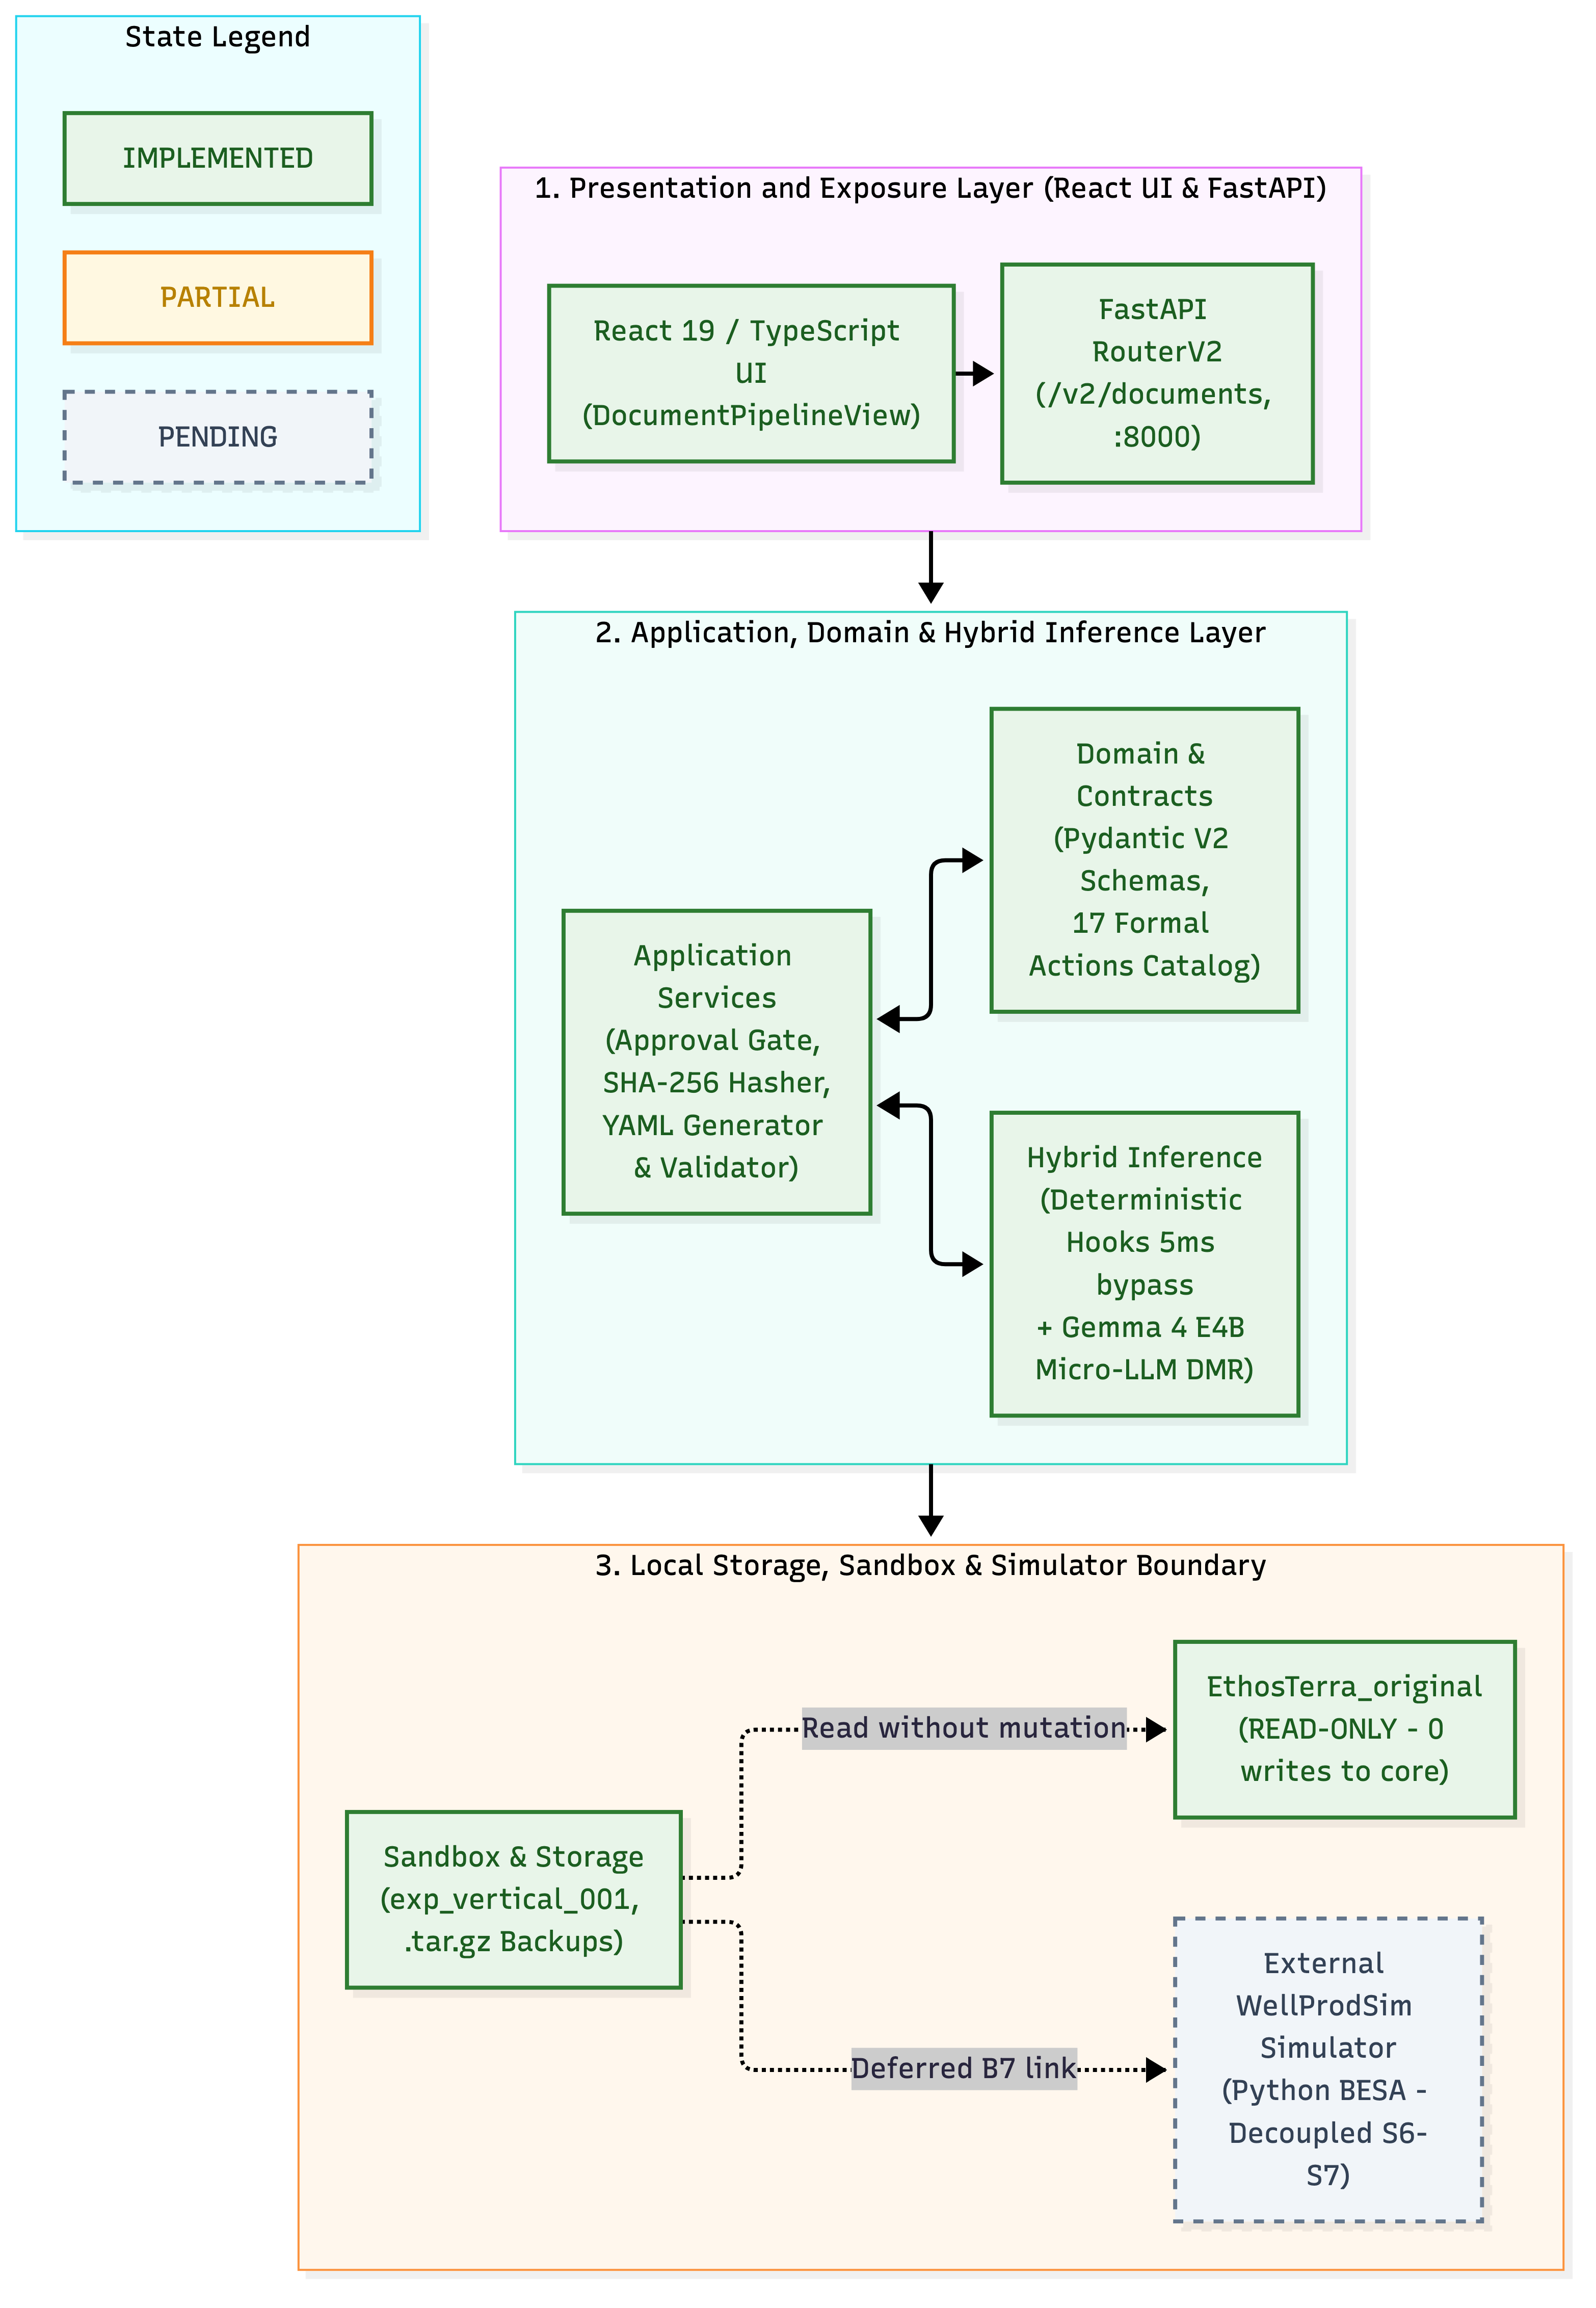
\includegraphics[width=0.92\textwidth,height=0.45\textheight,keepaspectratio]{figures/en/d01_arch_layers_en.png}
    \caption{Figure D1. Layered System Architecture. Illustrates the clean decoupling between UI, REST API, domain layer, local model runtime, and the simulation boundary.}
    \label{fig:d01_arch_layers}
\end{figure}

To precisely delineate the boundary of Block B5, Figure~\ref{fig:d12_b5_boundary} illustrates the read and write boundaries of the manual CRUD. The service operates strictly within the \texttt{outputs/intents/} store, enforcing an absolute barrier against \texttt{EthosTerra\_original/}.

\begin{figure}[H]
    \centering
    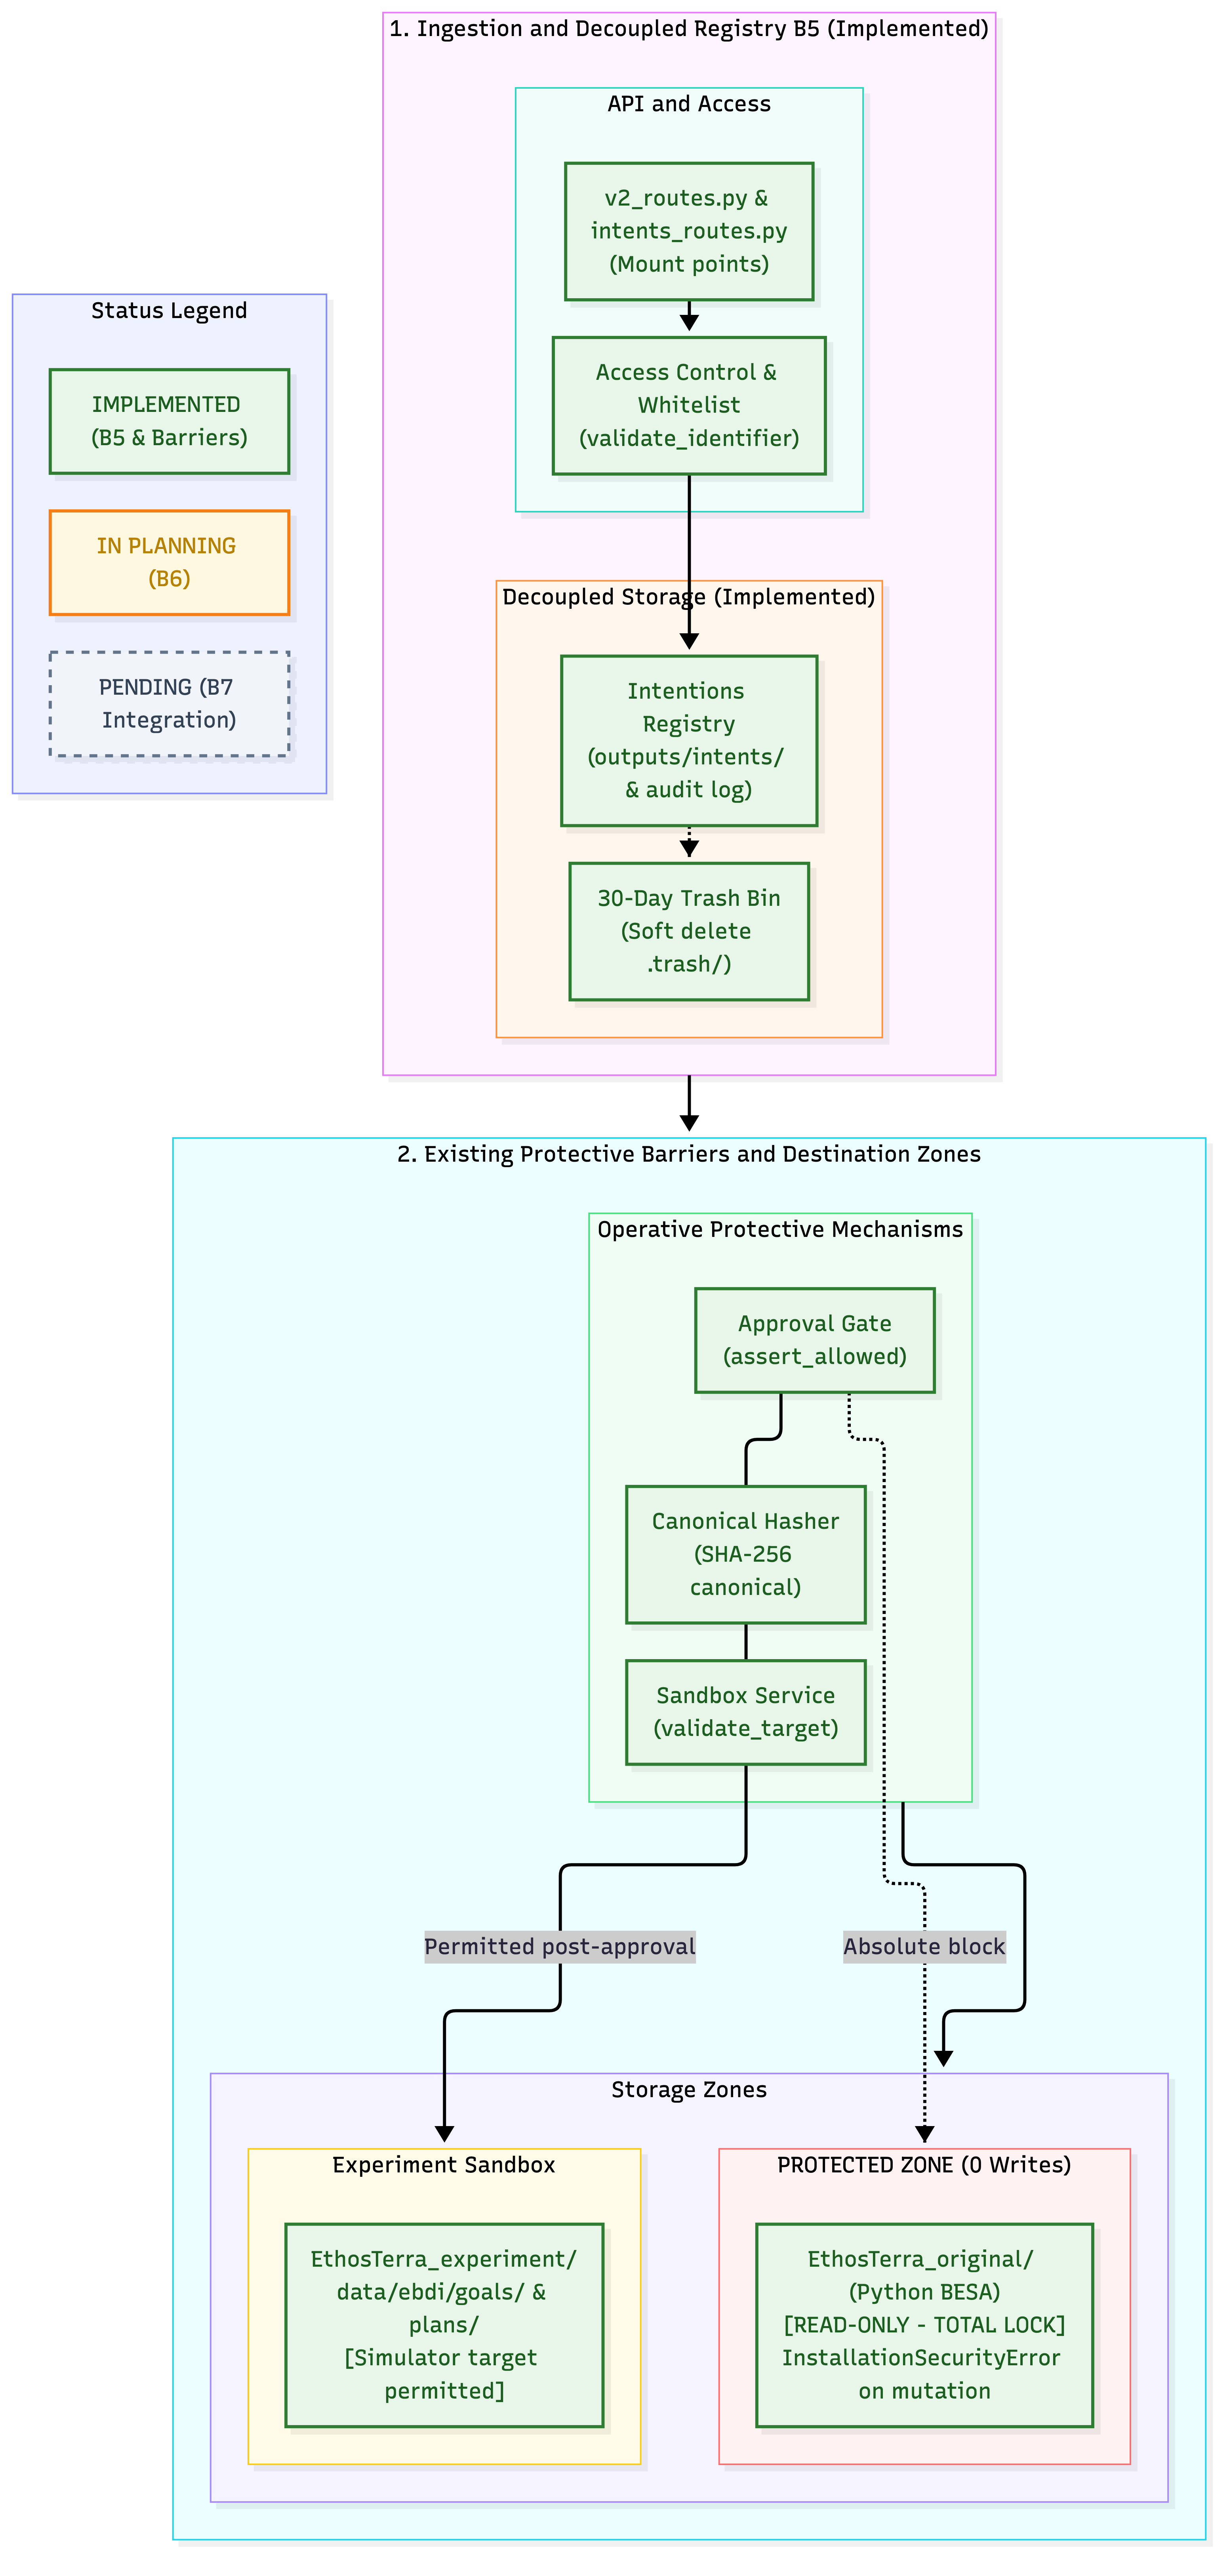
\includegraphics[width=0.92\textwidth,height=0.45\textheight,keepaspectratio]{figures/en/d12_b5_boundary_en.png}
    \caption{Figure D12. Functional and Security Boundary of Block B5. Highlights active store, 30-day trash, audit log, and containment barriers protecting the external simulation core.}
    \label{fig:d12_b5_boundary}
\end{figure}

Furthermore, the C4 component structure supporting backend orchestration is depicted in Figure~\ref{fig:d03_c4_components}.

\begin{figure}[H]
    \centering
    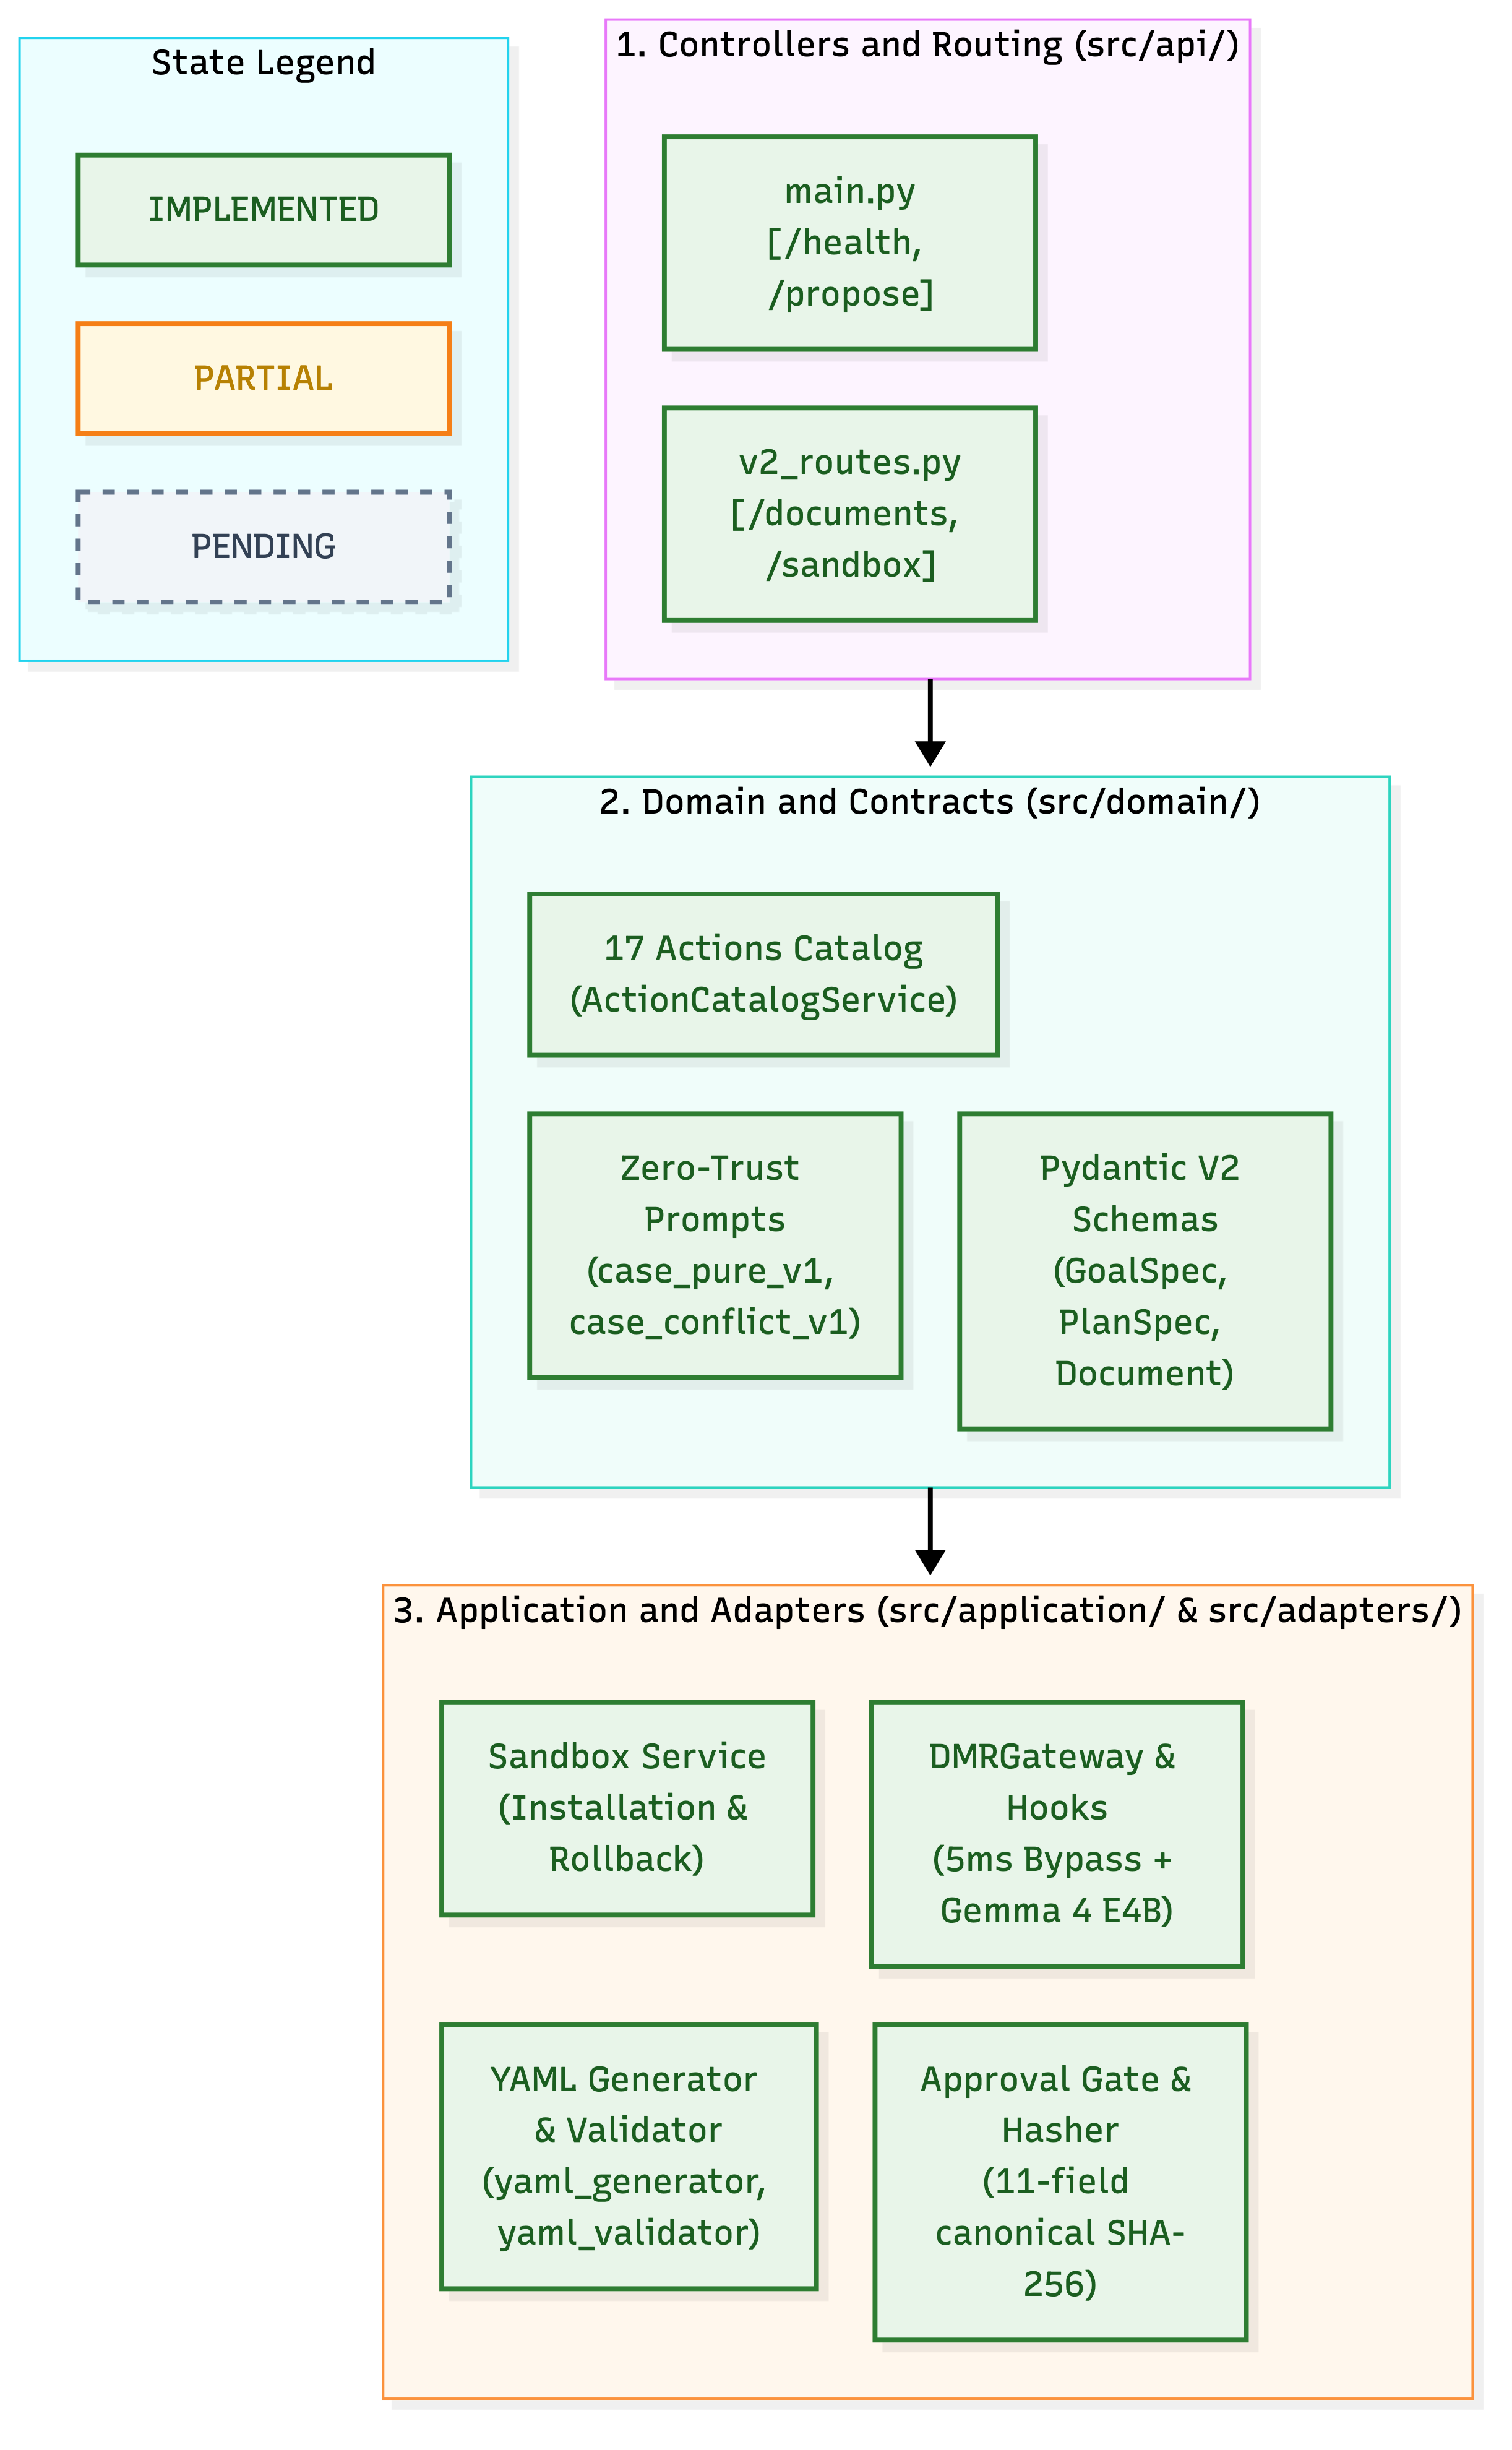
\includegraphics[width=0.92\textwidth,height=0.45\textheight,keepaspectratio]{figures/en/d03_c4_components_en.png}
    \caption{Figure D3. C4 Component Diagram of the FastAPI Backend, showing the injection of \texttt{ManualIntentService} and its filesystem adapters.}
    \label{fig:d03_c4_components}
\end{figure}

% ==============================================================================
% 10. TECHNICAL DEVELOPMENT
% ==============================================================================
\section{Technical Development}

\subsection{Data Model and Pydantic V2 Validation}
The file \texttt{apps/api/src/domain/v2/intent\_schemas.py} defines the DTO contracts for B5. The intention payload (\texttt{intent}) employs a discriminated union based on the literal field \texttt{tipo}:
\begin{lstlisting}[language=Python]
IntentPayload = Annotated[CasoPuro | CasoConflictivo, Field(discriminator="tipo")]

class CreateIntentRequest(BaseModel):
    model_config = ConfigDict(extra="forbid", str_strip_whitespace=True)
    id: str = Field(..., description="Unique alphanumeric ID (1-64 chars)")
    author: str = Field(default="operador_manual", min_length=1, max_length=64)
    intent: IntentPayload

class UpdateIntentRequest(BaseModel):
    model_config = ConfigDict(extra="forbid", str_strip_whitespace=True)
    author: str = Field(default="operador_manual", min_length=1, max_length=64)
    intent: IntentPayload
\end{lstlisting}

Figure~\ref{fig:d08_data_model} summarizes the formal schemas and contracts governing Pure and Conflict Cases.

\begin{figure}[H]
    \centering
    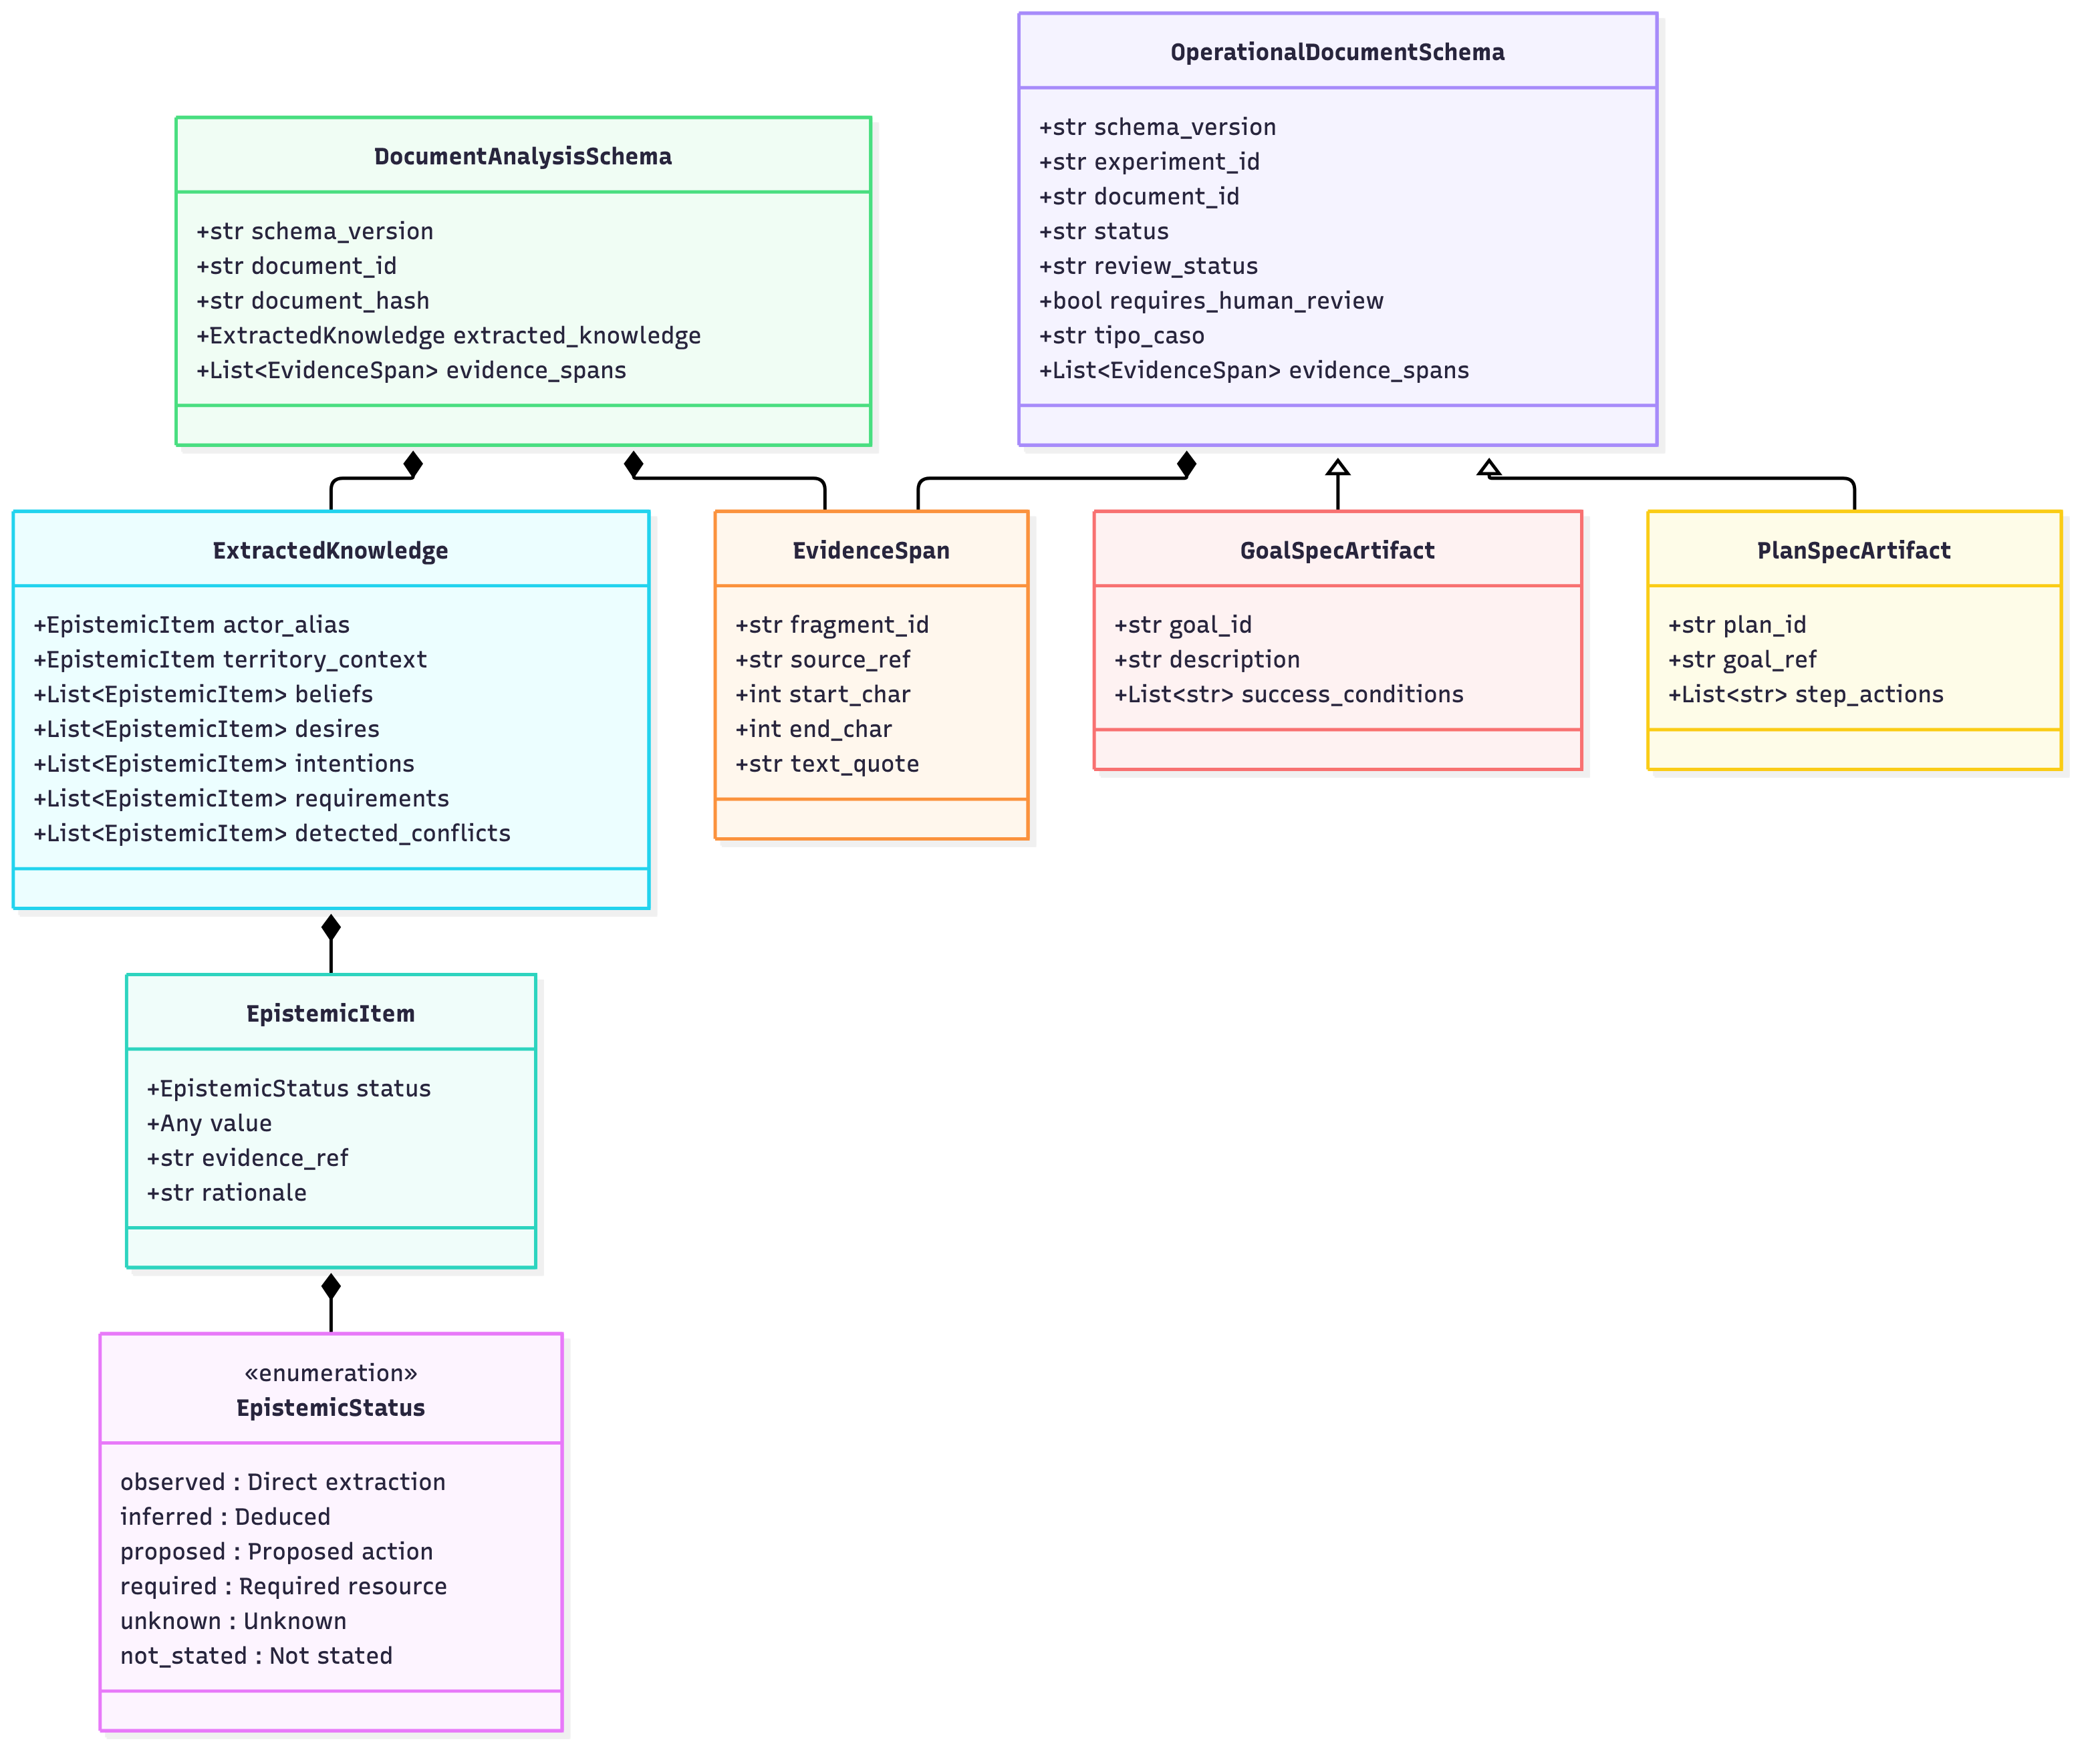
\includegraphics[width=0.92\textwidth,height=0.45\textheight,keepaspectratio]{figures/en/d08_data_model_contracts_en.png}
    \caption{Figure D8. Data Model and Formal Contracts. Schema structures for Pure Case (\texttt{CasoPuro}) and Conflict Case (\texttt{CasoConflictivo}).}
    \label{fig:d08_data_model}
\end{figure}

\subsection{Atomic Persistence and Disk Resilience}
The \texttt{ManualIntentService} (\texttt{apps/api/src/application/manual\_intent\_service.py}) guarantees atomic writes to disk following POSIX standards:
\begin{enumerate}
    \item Writes to a unique temporary file (\texttt{temp\_path}) appending a random UUID suffix (\texttt{.tmp.<hex>}).
    \item Forces userspace buffer flush and kernel disk block synchronization via \texttt{f.flush()} and \texttt{os.fsync(f.fileno())}.
    \item Renames the file atomically via POSIX filesystem swap using \texttt{os.replace(temp\_path, target\_path)}.
    \item A \texttt{finally} block guarantees deletion of the temporary file if any exception occurs prior to rename, preventing partial writes from corrupting the active store.
\end{enumerate}

\subsection{Soft Delete and 30-Day Retention Window}
Invoking \texttt{DELETE /v2/intents/\{id\}} does not purge the file. The record is parsed, enriched with the \texttt{trash\_metadata} block:
\begin{lstlisting}[language=Python]
trash_meta = {
    "deleted_at": datetime.now(timezone.utc).isoformat(),
    "deleted_by": deleted_by,
    "retention_days": 30,
    "expires_at": (datetime.now(timezone.utc) + timedelta(days=30)).isoformat(),
    "is_expired": False
}
\end{lstlisting}
and atomically moved to \texttt{outputs/intents/.trash/\{id\}.json}. During this window, records can be restored (\texttt{POST /v2/intents/\{id\}/restore}). If an item exceeds \texttt{expires\_at}, restoration attempts return \textbf{HTTP 410 Gone}.

\subsection{Scheduled Purge of Expired Records}
Permanent disk deletion occurs on-demand via \texttt{POST /v2/intents/trash/purge} (or \texttt{make purge-trash}) and automatically during FastAPI application startup via a lifespan hook in \texttt{src/api/main.py}. Files are purged only when \texttt{now >= expires\_at} evaluates to true.

% ==============================================================================
% 11. IMPLEMENTATION RESULTS
% ==============================================================================
\section{Implementation Results}

\subsection{REST Endpoints Exposed}
The REST router registered under \texttt{/v2/intents} provides eight fully tested operations:
\begin{itemize}[itemsep=1pt]
    \item \texttt{POST /v2/intents}: Strict creation (HTTP 201). Rejects duplicates with HTTP 409.
    \item \texttt{GET /v2/intents}: Consolidated listing of active intentions (HTTP 200).
    \item \texttt{GET /v2/intents/\{id\}}: Retrieval by unique alphanumeric identifier (HTTP 200 / 404).
    \item \texttt{PUT /v2/intents/\{id\}}: Versioned update computing new SHA-256 hash (HTTP 200 / 404 / 422).
    \item \texttt{DELETE /v2/intents/\{id\}}: Soft-delete moving record to \texttt{.trash/} (HTTP 200 / 404).
    \item \texttt{GET /v2/intents/trash}: Listing of items in trash with expiration metadata (HTTP 200).
    \item \texttt{POST /v2/intents/\{id\}/restore}: Restoration to active store (HTTP 200 / 409 / 410).
    \item \texttt{POST /v2/intents/trash/purge}: Permanent purge of records older than 30 days (HTTP 200).
\end{itemize}

\subsection{React Web User Interface}
The \texttt{ManualIntentsView.tsx} component integrates seamlessly into the Vite dashboard:
\begin{itemize}[itemsep=2pt]
    \item \textbf{Live KPI Header:} Real-time counters for active intentions, Pure vs. Conflict breakdown, trash count, and backend API connectivity.
    \item \textbf{1-Click Agronomic Templates:} Instant pre-loading of compliant structures for conservation tillage (Pure) and irrigation quota dilemmas (Conflict).
    \item \textbf{30-Day Trash Manager:} Visual progress bar showing remaining retention days before permanent purge and instant restore button.
    \item \textbf{Build and Static Analysis:} Production bundle compiled with Vite in 213~ms; static analysis via \texttt{oxlint} in 26~ms with 0 errors and 0 warnings.
\end{itemize}

The web interface was executed and manually inspected in the local browser. The creation, retrieval, editing, logical deletion, trash inspection, restoration, and purge workflows were verified. The display of Pure Case and Conflict Case records, including their specific fields and API response messages, was also checked. The observed flows matched the expected behavior defined for Block B5.

% ==============================================================================
% 12. AUDIT RESULTS
% ==============================================================================
\section{Audit Results}

The formal technical audit was executed reproducibly against an isolated temporary directory (\texttt{tmp\_path}). Table~\ref{tab:matriz_b5_en} details the acceptance matrix across criteria B5-01 through B5-24:

\begin{table}[H]
\centering
\small
\begin{tabularx}{\textwidth}{p{1.1cm}p{3.3cm}Xp{1.5cm}p{3.2cm}}
\toprule
\textbf{ID} & \textbf{Criterion} & \textbf{Required Evidence} & \textbf{Status} & \textbf{Remarks} \\
\midrule
B5-01 & Create Pure Case & POST HTTP 201, atomic disk persistence & PASS & Version 1, canonical hash \\
B5-02 & Create Conflict Case & POST HTTP 201, validated contract & PASS & Colliding sources intact \\
B5-03 & Validate Invalid Data & HTTP 422 on extra or malformed fields & PASS & \texttt{extra="forbid"} enforced \\
B5-04 & Prevent Overwrite & HTTP 409 on duplicate identifier & PASS & Existing file untouched \\
B5-05 & Update Intention & PUT HTTP 200 with incremented version & PASS & Version increments 1 to 2 \\
B5-06 & Invalid Update & HTTP 422 on malformed payload & PASS & Pre-existing file preserved \\
B5-07 & List and Retrieve & GET HTTP 200 on read endpoints & PASS & Payload integrity preserved \\
B5-08 & Soft Delete & Relocation to \texttt{.trash/} with metadata & PASS & 100\% soft delete (4/4) \\
B5-09 & 30-Day Retention & Block purge if $t < 30\text{d}$ & PASS & Simulated time verified \\
B5-10 & Purge Expired & Physical deletion if $t \ge 30\text{d}$ & PASS & Permanent purge verified \\
B5-11 & Restore Intention & Reintegration into active directory & PASS & Record removed from trash \\
B5-12 & Restore Conflict & HTTP 409 if active ID exists & PASS & Collision detected cleanly \\
B5-13 & Path Traversal Block & 100\% rejection of negative cases (5/5) & PASS & Strict regex whitelist \\
B5-14 & Symlink Block & HTTP 403 on symbolic link target & PASS & \texttt{Path.is\_symlink()} check \\
B5-15 & Confined Writes & Confined to \texttt{outputs/intents/} & PASS & Prefix validation enforced \\
B5-16 & Atomic Write Faults & Failure in \texttt{os.replace} preserves state & PASS & Base file uncorrupted \\
B5-17 & Orphaned Temps & 0 temporary files after forced failure & PASS & \texttt{finally} cleanup verified \\
B5-18 & Audit Trail & Append-only entries in \texttt{audit.log} & PASS & 14/14 events registered \\
B5-19 & Hash Integrity & Deterministic canonical SHA-256 & PASS & Normalized key sorting \\
B5-20 & Protected Core & 0 writes to external simulation core & PASS & 514 files, hash identical \\
B5-21 & API Status Codes & Responses 200, 201, 403, 404, 409, 410, 422 & PASS & Automated TestClient suite \\
B5-22 & User Interface & Code, TypeScript contracts, build, lint, HTTP tests, and manual browser validation & PASS & Flows match B5 design specifications \\
B5-23 & Non-Regression & Global monorepo suite runs without failure & PASS & 79/79 unit tests passed \\
B5-24 & Git Governance & Working tree clean, zero unauthorized commits & PASS & Rules 9 and 10 observed \\
\bottomrule
\end{tabularx}
\caption{Acceptance Matrix for Block B5. Functional, security, and persistence criteria verification.}
\label{tab:matriz_b5_en}
\end{table}

% ==============================================================================
% 13. SECURITY AND TRACEABILITY
% ==============================================================================
\section{Security and Traceability}

\subsection{Negative Input Validation}
A \textbf{100\% rejection rate was achieved across the 16 evaluated negative test cases} (16/16). Table~\ref{tab:casos_negativos_en} categorizes each test vector, the resulting HTTP status code, and the active mitigation mechanism.

\begin{table}[H]
\centering
\small
\begin{tabularx}{\textwidth}{llccX}
\toprule
\textbf{\#} & \textbf{Evaluated Negative Case} & \textbf{HTTP} & \textbf{Status} & \textbf{Mitigation Mechanism} \\
\midrule
1 & Empty identifier (\texttt{""}) & 422 & PASS & Pydantic minimum length validation \\
2 & Identifier with internal whitespace & 422 & PASS & Regex pattern whitelist rejection \\
3 & Path traversal sequence (\texttt{../}) & 422 & PASS & Escape sequence pattern detection \\
4 & POSIX directory separator (\texttt{/}) & 422 & PASS & Hierarchy delimiter prohibition \\
5 & Windows path separator (\texttt{\textbackslash}) & 422 & PASS & Backslash character prohibition \\
6 & Absolute filesystem path (\texttt{/etc/intent}) & 422 & PASS & Leading slash character rejection \\
7 & Forced symbolic link target & 403 & PASS & Explicit check via \texttt{is\_symlink()} \\
8 & Identifier exceeding 64 characters & 422 & PASS & Strict boundary \texttt{max\_length=64} \\
9 & Payload containing undeclared fields & 422 & PASS & Pydantic \texttt{extra="forbid"} \\
10 & Payload missing mandatory fields & 422 & PASS & Discriminator block validation \\
11 & Invalid case discriminator (\texttt{magico}) & 422 & PASS & Union literal constraint (\texttt{puro}/\texttt{conflicto}) \\
12 & Update on non-existent identifier & 404 & PASS & Handled via \texttt{IntentNotFoundError} \\
13 & Delete on non-existent identifier & 404 & PASS & Pre-existence validation check \\
14 & Restore of non-existent trash record & 404 & PASS & Absence verified in \texttt{.trash/} \\
15 & Restore of expired record ($>30\text{d}$) & 410 & PASS & Temporal expiration check \\
16 & Duplicate identifier creation & 409 & PASS & Handled via \texttt{FileExistsError} \\
\bottomrule
\end{tabularx}
\caption{Negative Input Validation Results in Block B5.}
\label{tab:casos_negativos_en}
\end{table}

\subsection{Cryptographic Verification of the Protected Core}
To confirm that the CRUD subsystem does not alter the production simulation core, the external repository directory was directly inspected:
\begin{center}
\texttt{/Volumes/ADATA SD620/Programacion 7.0/universidad/proyecto de grado/EthosTerra}
\end{center}
This directory hosts the standalone Python BESA simulation framework, scenario scripts, and reference documentation. The verification was conducted using the following reproducible commands:
\begin{lstlisting}[language=bash]
# Inventory of regular files
find "/Volumes/ADATA SD620/Programacion 7.0/universidad/proyecto de grado/EthosTerra" -type f | wc -l
# Deterministic combined SHA-256 calculation
python3 -c '
import hashlib, sys
from pathlib import Path
target = Path("/Volumes/ADATA SD620/Programacion 7.0/universidad/proyecto de grado/EthosTerra")
files = sorted([p for p in target.rglob("*") if p.is_file()])
h = hashlib.sha256()
for f in files:
    h.update(str(f.relative_to(target)).encode("utf-8"))
    h.update(f.read_bytes())
print(f"Total: {len(files)} files | Hash: {h.hexdigest()}")
'
\end{lstlisting}

\textbf{Comparative Audit Results:}
\begin{itemize}[itemsep=1pt]
    \item Total regular files before tests: \textbf{514}
    \item Total regular files after tests: \textbf{514}
    \item SHA-256 hash before: {\scriptsize\texttt{f182c62ebeb1bc85b49b3975366bf56ed062af775ed91ac63d0ef9ce65537a8a}}
    \item SHA-256 hash after: {\scriptsize\texttt{f182c62ebeb1bc85b49b3975366bf56ed062af775ed91ac63d0ef9ce65537a8a}}
    \item Conclusion: \textbf{$\text{core\_writes} = 0$}. 100\% of files remained strictly immutable.
\end{itemize}

% ==============================================================================
% 14. METRICS
% ==============================================================================
\section{Metrics}

\subsection{Quantitative Metrics of Block B5}
Table~\ref{tab:metricas_b5_en} reports quantitative audit metrics with explicit mathematical denominators.

\begin{table}[H]
\centering
\small
\begin{tabularx}{\textwidth}{p{4.2cm}Xccr}
\toprule
\textbf{Evaluation Metric} & \textbf{Calculation Formula} & \textbf{Num. / Den.} & \textbf{Percentage} & \textbf{Target} \\
\midrule
Valid creation rate & Successful creations / Valid attempts & 2 / 2 & 100.0\% & 100\% \\
Negative rejection rate & Compliant rejections / Negative cases & 16 / 16 & 100.0\% & 100\% \\
Versioned update rate & Successful updates / Valid attempts & 2 / 2 & 100.0\% & 100\% \\
Soft-delete rate & Soft deletes / Normal deletions & 4 / 4 & 100.0\% & 100\% \\
30-day retention rate & Enforced retentions / Cases $<30\text{d}$ & 2 / 2 & 100.0\% & 100\% \\
Expired purge rate & Purged records / Cases $\ge 30\text{d}$ & 2 / 2 & 100.0\% & 100\% \\
Restoration rate & Successful restorations / Valid attempts & 2 / 2 & 100.0\% & 100\% \\
Path traversal block rate & Blocked escapes / Path attacks & 5 / 5 & 100.0\% & 100\% \\
Symlink block rate & Blocked links / Symlink attacks & 1 / 1 & 100.0\% & 100\% \\
Atomicity fault rate & Faults without orphans / Induced faults & 3 / 3 & 100.0\% & 100\% \\
Audit traceability rate & Logged events / Executed mutations & 14 / 14 & 100.0\% & 100\% \\
Simulation core writes & Created + Modified + Deleted files & 0 / 514 & 0 & 0 \\
\bottomrule
\end{tabularx}
\caption{Quantitative Metrics for Security, Persistence, and Operation in Block B5.}
\label{tab:metricas_b5_en}
\end{table}

\subsection{Classification of Experimental Evidence by Origin}
Table~\ref{tab:origen_evidencia_en} delineates evidence generated during Week 8 from inherited baseline components.

\begin{table}[H]
\centering
\small
\begin{tabularx}{\textwidth}{lp{5.0cm}p{4.2cm}l}
\toprule
\textbf{Category} & \textbf{Evaluated Components} & \textbf{Verification Method} & \textbf{Status} \\
\midrule
\textbf{Week 8 (B5)} & Manual CRUD, trash, 30d retention, purge, atomicity, hash, UI & 26 B5 tests, isolated testbed, core inventory & Validated \\
\textbf{Inherited (W5--W7)} & Approval Gate, hybrid classifier, domain hooks, sandbox exp\_001 & 53 baseline tests, Week 5 report & Immutable \\
\textbf{Static Inspection} & Pydantic V2 contracts, identifier regex, UI linter & \texttt{extra="forbid"}, \texttt{oxlint} (26ms), \texttt{tsc -b} & Pass \\
\textbf{Automated Testing} & REST endpoints, HTTP status codes, lifecycle & \texttt{TestClient}, \texttt{pytest} (79 tests in 0.35s) & Pass \\
\textbf{Browser Inspection} & User experience and B5 flows & Inspection at \texttt{localhost:5173} & Pass \\
\bottomrule
\end{tabularx}
\caption{Classification and Separation of Experimental Evidence by Origin.}
\label{tab:origen_evidencia_en}
\end{table}

\subsection{Visual Chart of Automated Test Results}
Figure~\ref{fig:chart_tests_en} summarizes the distribution of automated tests executed during the technical audit.

\begin{figure}[H]
\centering
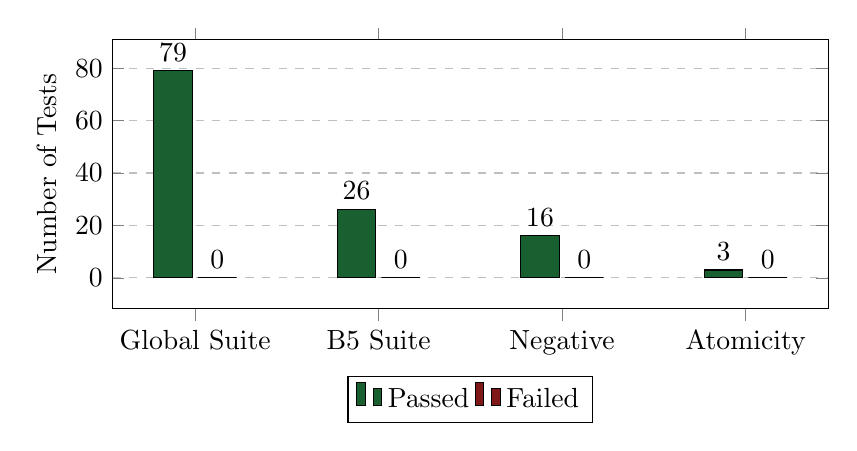
\begin{tikzpicture}
\begin{axis}[
    ybar,
    bar width=14pt,
    width=0.88\textwidth,
    height=5.0cm,
    enlargelimits=0.15,
    ylabel={Number of Tests},
    symbolic x coords={Global Suite, B5 Suite, Negative, Atomicity},
    xtick=data,
    nodes near coords,
    nodes near coords align={vertical},
    legend style={at={(0.5,-0.25)}, anchor=north, legend columns=-1},
    ymajorgrids=true,
    grid style=dashed
]
\addplot[fill=darkgreen!80!black] coordinates {(Global Suite, 79) (B5 Suite, 26) (Negative, 16) (Atomicity, 3)};
\addplot[fill=warnred!80!black] coordinates {(Global Suite, 0) (B5 Suite, 0) (Negative, 0) (Atomicity, 0)};
\legend{Passed, Failed}
\end{axis}
\end{tikzpicture}
\caption{Distribution of Automated Tests Passed versus Failed.}
\label{fig:chart_tests_en}
\end{figure}

The state machine governing the lifecycle of manual intentions is illustrated in Figure~\ref{fig:lifecycle_diagram_en}.

\begin{figure}[H]
\centering
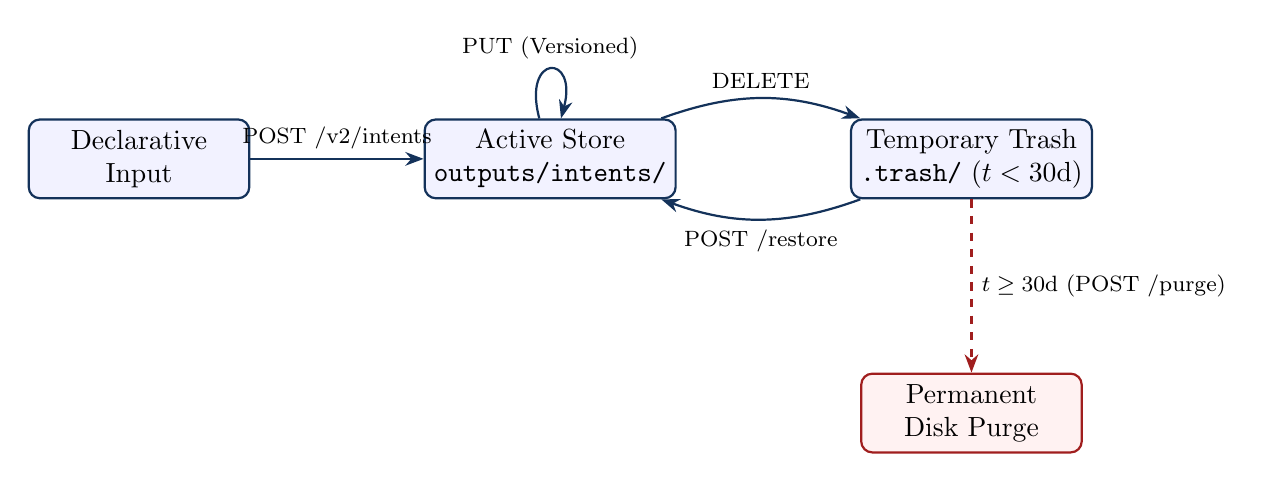
\begin{tikzpicture}[
    node distance=2.2cm,
    state/.style={rectangle, rounded corners, draw=navyblue, fill=blue!5, thick, minimum width=2.8cm, minimum height=1.0cm, align=center},
    edge/.style={->, >=Stealth, thick, draw=navyblue},
    warnedge/.style={->, >=Stealth, thick, draw=warnred, dashed}
]
\node[state] (nuevo) {Declarative\\Input};
\node[state, right=of nuevo] (activo) {Active Store\\\texttt{outputs/intents/}};
\node[state, right=of activo] (papelera) {Temporary Trash\\\texttt{.trash/} ($t < 30\text{d}$)};
\node[state, below=of papelera, draw=warnred, fill=red!5] (purgado) {Permanent\\Disk Purge};

\draw[edge] (nuevo) -- node[above]{\footnotesize POST /v2/intents} (activo);
\draw[edge] (activo) to[bend left=20] node[above]{\footnotesize DELETE} (papelera);
\draw[edge] (papelera) to[bend left=20] node[below]{\footnotesize POST /restore} (activo);
\draw[warnedge] (papelera) -- node[right]{\footnotesize $t \ge 30\text{d}$ (POST /purge)} (purgado);
\draw[edge] (activo) to[loop above] node[above]{\footnotesize PUT (Versioned)} (activo);
\end{tikzpicture}
\caption{Persistence Lifecycle State Machine: Active Store, Temporary Trash, and Permanent Purge.}
\label{fig:lifecycle_diagram_en}
\end{figure}

% ==============================================================================
% 15. DISCUSSION
% ==============================================================================
\section{Discussion}

The architecture implemented in Block B5 corroborates the hypothesis that industrial-grade robustness and forensic traceability can be achieved without introducing accidental complexity. Relying on local JSON files backed by POSIX atomic filesystem primitives (\texttt{os.replace}) eliminated the need for SQL database engines or in-memory key-value stores (e.g., Redis), reducing external network dependencies to zero and preserving a strictly offline-first execution profile.

A critical design observation highlighted by the audit relates to Pydantic V2 contract strictness: enforcing \texttt{extra="forbid"} deterministically rejects any client request containing misspelled or extraneous fields (such as submitting \texttt{"created\_by"} instead of \texttt{"author"}), returning HTTP 422. Similarly, in Conflict Cases, restricting colliding sources to domain literals (\texttt{"context\_field"} and \texttt{"document"}) prevents unstructured narrative descriptions from degrading the semantic rigor of the eBDI arbitration gate.

% ==============================================================================
% 16. LIMITACIONES (LIMITATIONS)
% ==============================================================================
\section{Limitations}

The following scope considerations apply to the current engineering increment:
\begin{enumerate}[itemsep=2pt]
    \item \textbf{Simulator integration deferred to Block B7:} Block B5 focuses on local declarative persistence; active integration with the deliberative cycle of the WellProdSim / EthosTerra multi-agent simulator is scheduled for Weeks 10 through 12.
    \item \textbf{Comprehensive simulation testing scheduled for Block B9:} Full end-to-end simulation runs verifying dynamic agent belief mutations belong formally to Block B9 (Weeks 12 and 13).
    \item \textbf{Trash purge coupled to API startup or manual trigger:} To avoid unmanaged background daemons, permanent disk purging is executed during FastAPI startup (via lifespan hook) or upon explicit REST endpoint invocation.
    \item \textbf{Simulation core verification dependent on local volume mounting:} Physical verification of zero writes against \texttt{EthosTerra} depends on the availability of the mounted volume on the host; in environments without it, safety is enforced via static path containment assertions in the codebase.
    \item \textbf{Expert panel evaluation scheduled for Block B10:} Formal semantic validation with rural extensionists and agronomic experts is planned for Block B10 (Weeks 13 and 14).
\end{enumerate}

% ==============================================================================
% 17. STATUS AGAINST ROADMAP
% ==============================================================================
\section{Status Against Roadmap}

The consolidated development roadmap encompassing all thirteen project blocks is illustrated in Figure~\ref{fig:d11_roadmap}. Block B5 is successfully concluded within its allocated timeframe (Weeks 8 and 9).

\begin{figure}[H]
    \centering
    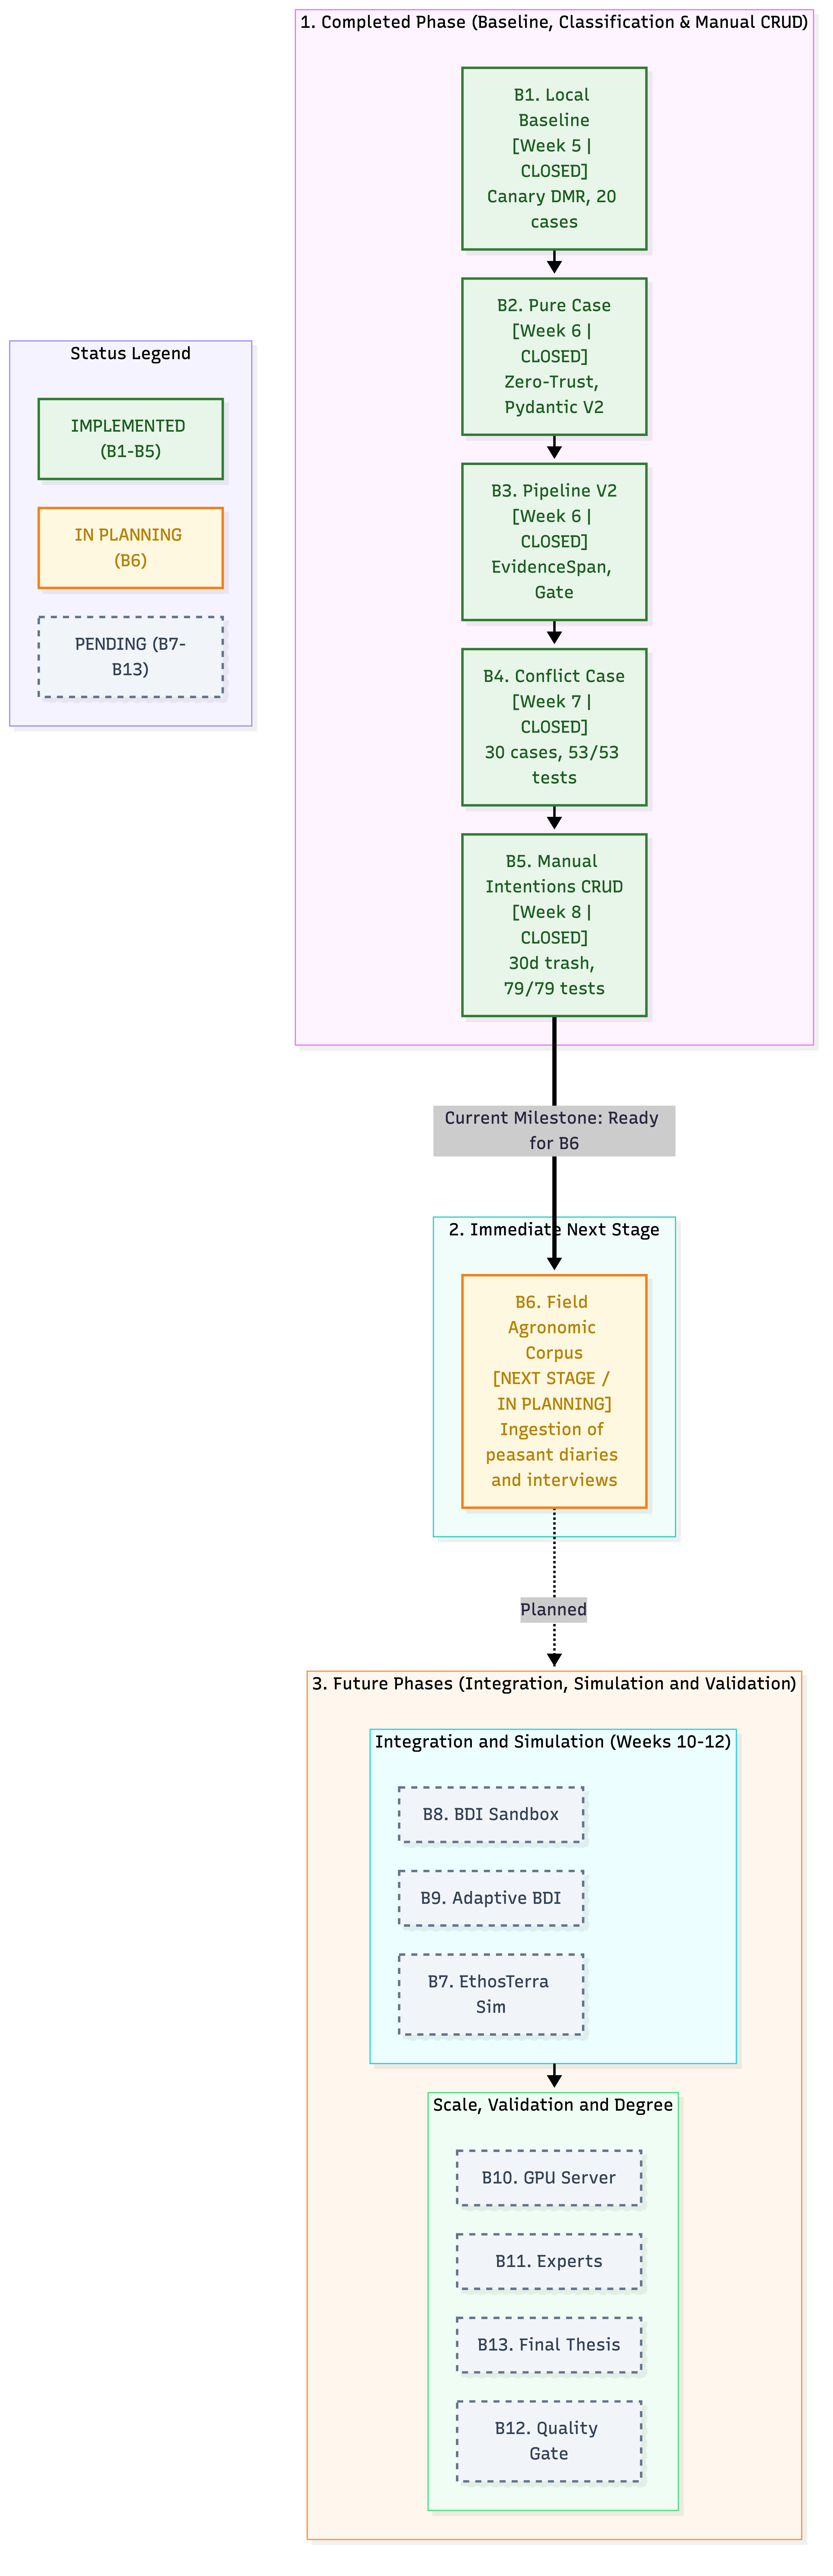
\includegraphics[width=0.92\textwidth,height=0.45\textheight,keepaspectratio]{figures/en/d11_status_roadmap_en.png}
    \caption{Figure D11. Project Status Map and Development Roadmap (Blocks B1 through B13), marking the completion of Block B5 and transition to Block B6.}
    \label{fig:d11_roadmap}
\end{figure}

The formal milestone status according to the Phase 2 research schedule is outlined in Table~\ref{tab:cronograma_en}.

\begin{table}[H]
\centering
\small
\begin{tabularx}{\textwidth}{p{1.8cm}p{4.5cm}ccX}
\toprule
\textbf{Block} & \textbf{Technical Description} & \textbf{Weeks} & \textbf{Formal Status} & \textbf{Remarks} \\
\midrule
\textbf{B1--B3} & Pure Case Classifier & 1--5 & Closed & 20 cases evaluated with Gemma 4 \\
\textbf{B4} & Conflict Case Classifier & 6--7 & Closed & Collision matrix and Week 7 report \\
\textbf{B5} & Manual Intentions CRUD & 8--9 & \textbf{Completed} & Audit and manual inspection passed \\
\textbf{B6} & Agronomic Corpus Testing & 9--10 & Pending & Field journal ingestion \\
\textbf{B7} & Simulator Integration & 10--12 & Pending & Python BESA connection \\
\textbf{B8} & Multi-Agent eBDI System & 4--11 & In parallel & Goal and plan modeling \\
\textbf{B9} & End-to-End Simulation Tests & 12--13 & Pending & Full simulation with rollback \\
\textbf{B10} & Internal Semantic Validation & 13--14 & Pending & Expert panel preparation \\
\textbf{B11--B13} & Thesis Consolidation & 14--16 & Pending & Master's thesis delivery \\
\bottomrule
\end{tabularx}
\caption{Current Progress of the Semester Research Schedule (Phase 2).}
\label{tab:cronograma_en}
\end{table}

% ==============================================================================
% 18. PENDING WORK
% ==============================================================================
\section{Pending Work}

To formally transition to Block B6, the following tasks are established:
\begin{enumerate}[itemsep=2pt]
    \item Execute the mandatory pre-commit check and request user authorization to freeze the Week 8 increment in Git.
    \item Collect and normalize the field journal corpus from smallholder agricultural contexts for the Block B6 evaluation suite.
    \item Design load and concurrency stress tests for the file-based intention store exceeding 100 concurrent files.
    \item Structure preliminary integration interfaces for Block B7 against Python BESA.
\end{enumerate}

% ==============================================================================
% 19. CONCLUSIONS
% ==============================================================================
\section{Conclusions}

Week 8 completed Block B5 of the project. The manual intent CRUD is functional for Pure and Conflict Cases, including JSON persistence, version control, logical deletion, retention, restoration, purge, input validation, atomic writing, auditing, and path protection. Automated tests and manual inspection of the web interface confirmed the expected behavior. The block is therefore completed, while the next activities correspond to the integration and testing tasks scheduled for subsequent weeks.

The official milestone verdict is \textbf{B5 COMPLETED}.

% ==============================================================================
% 20. REFERENCES
% ==============================================================================
\section{References}

\begin{enumerate}[itemsep=2pt]
    \item Bratman, M. (1987). \textit{Intentions, Plans, and Practical Reason}. Harvard University Press.
    \item Rao, A. S., \& Georgeff, M. P. (1995). BDI agents: From theory to practice. \textit{Proceedings of the First International Conference on Multi-Agent Systems (ICMAS-95)}, 312--319.
    \item WellProdSim Development Team. (2025). \textit{WellProdSim: Agronomic Multi-Agent Simulation Environment}. Internal Design Specifications.
    \item Martínez Velandia, J. A. (2026). \textit{Experimental Progress Report -- Week 7 (Block B4): Implementation of the Conflict Case Classifier}. Universidad Tecnológica de Bolívar.
    \item Pydantic Documentation. (2026). \textit{Data validation and settings management using Python type annotations}. Version 2.13.
    \item FastAPI Framework. (2026). \textit{High performance, easy to learn, fast to code, ready for production}.
\end{enumerate}

% ==============================================================================
% 21. TECHNICAL ANNEXES
% ==============================================================================
\section{Technical Annexes}

\subsection{Annex A: Operational Commands and Makefile}
To reproduce all tests and launch local services, the repository provides standardized targets in the \texttt{Makefile}:
\begin{lstlisting}[language=bash]
# Run B5 manual intentions test suite (26 tests)
make test-b5

# Run complete non-regression unit suite (79 tests)
make test-unit

# Start FastAPI backend (port 8000) and Vite frontend (port 5173) concurrently
make dev

# Purge expired trash intentions (>30 days) on demand
make purge-trash
\end{lstlisting}

\subsection{Annex B: Canonical Structure of a Persisted Conflict Case}
A real persisted file located at \texttt{outputs/intents/agro\_conflicto\_riego\_cuota.json} illustrates the canonical structure:
\begin{lstlisting}[basicstyle=\ttfamily\scriptsize]
{
  "id": "agro_conflicto_riego_cuota",
  "intent": {
    "tipo": "conflicto",
    "conflicto_detectado": "Incompatibilidad entre limite comunal de consumo hidrico y estres severo.",
    "opciones_resolucion": [
      "Respetar turno comunal y posponer riego a horas nocturnas",
      "Riego de socorro localizado por goteo",
      "Solicitar ampliacion temporal de cuota ante junta de regantes"
    ],
    "requiere_humano": true,
    "descripcion_contradiccion": "Dilema entre estres hidrico y veda comunal.",
    "fuentes_en_colision": [
      {
        "source_type": "context_field",
        "source_id": "soil_moisture_level",
        "intencion": "regar_inmediato",
        "efecto": "mitigar_estres_hidrico",
        "evidence_ref": "telemetria_sensor_p2"
      },
      {
        "source_type": "document",
        "source_id": "estatuto_riego_comunal",
        "intencion": "racionar_consumo",
        "efecto": "evitar_sancion_y_desabastecimiento",
        "evidence_ref": "estatuto_2026_cap3"
      }
    ],
    "confidence": 1.0,
    "razonamiento": "Contradiccion insalvable entre telemetria de campo y acuerdo comunitario."
  },
  "metadata": {
    "created_at": "2026-10-02T10:46:14.355624Z",
    "created_by": "revisor_normativo",
    "updated_at": "2026-10-02T10:46:14.355624Z",
    "updated_by": "revisor_normativo",
    "canonical_hash": "7a4814d0b2f557c8e3c6dc69c424441d1a6274f231a5bc94f9f9b61ffc6f70e6",
    "version": 1
  }
}
\end{lstlisting}

\subsection{Annex C: Document Compilation Instructions}
This document can be independently compiled using either of the following commands:
\begin{lstlisting}[language=bash]
# Option 1: Using latexmk (recommended)
latexmk -pdf -interaction=nonstopmode informe_semana_8_en.tex

# Option 2: Using direct pdflatex
pdflatex -interaction=nonstopmode informe_semana_8_en.tex
pdflatex -interaction=nonstopmode informe_semana_8_en.tex
\end{lstlisting}

\end{document}
